%%%%%%%%%%%%%%%%%%%%%%%%%%%%%%%%%%%%%%%%%
% Programming/Coding Assignment
% LaTeX Template
%
% This template has been downloaded from:
% http://www.latextemplates.com
%
% Original author:
% Ted Pavlic (http://www.tedpavlic.com)
%
% Note:
% The \lipsum[#] commands throughout this template generate dummy text
% to fill the template out. These commands should all be removed when 
% writing assignment content.
%
% This template uses a Perl script as an example snippet of code, most other
% languages are also usable. Configure them in the "CODE INCLUSION 
% CONFIGURATION" section.
%
%%%%%%%%%%%%%%%%%%%%%%%%%%%%%%%%%%%%%%%%%

%----------------------------------------------------------------------------------------
%	PACKAGES AND OTHER DOCUMENT CONFIGURATIONS
%----------------------------------------------------------------------------------------

\documentclass{article}

\usepackage{fancyhdr} % Required for custom headers
\usepackage{lastpage} % Required to determine the last page for the footer
\usepackage{extramarks} % Required for headers and footers
\usepackage[usenames,dvipsnames]{color} % Required for custom colors
\usepackage{graphicx} % Required to insert images
\usepackage{listings} % Required for insertion of code
\usepackage{courier} % Required for the courier font
\usepackage{lipsum} % Used for inserting dummy 'Lorem ipsum' text into the template
\usepackage{setspace}
\usepackage{color}
\usepackage{comment}
\usepackage{caption}

\usepackage{hyperref}
\usepackage{natbib}
\usepackage{underscore}
\usepackage{subfigure}
\usepackage{fixltx2e}

\hypersetup{
    colorlinks=true,
    linkcolor=blue,
    filecolor=magenta,      
    urlcolor=cyan,
    breaklinks=true
}

%\usepackage[]{algorithm2e}
\usepackage{pdfpages}




%For python inclusion (http://widerin.org/blog/syntax-highlighting-for-python-scripts-in-latex-documents)
\definecolor{Code}{rgb}{0,0,0}
\definecolor{Decorators}{rgb}{0.5,0.5,0.5}
\definecolor{Numbers}{rgb}{0.5,0,0}
\definecolor{MatchingBrackets}{rgb}{0.25,0.5,0.5}
\definecolor{Keywords}{rgb}{0,0,1}
\definecolor{self}{rgb}{0,0,0}
\definecolor{Strings}{rgb}{0,0.63,0}
\definecolor{Comments}{rgb}{0,0.63,1}
\definecolor{Backquotes}{rgb}{0,0,0}
\definecolor{Classname}{rgb}{0,0,0}
\definecolor{FunctionName}{rgb}{0,0,0}
\definecolor{Operators}{rgb}{0,0,0}
\definecolor{Background}{rgb}{0.98,0.98,0.98}

% Margins
\topmargin=-0.45in
\evensidemargin=0in
\oddsidemargin=0in
\textwidth=6.5in
\textheight=9.0in
\headsep=0.25in

\linespread{1.1} % Line spacing

% Set up the header and footer
\pagestyle{fancy}
\lhead{\hmwkAuthorName} % Top left header
%\chead{\hmwkClass\ (\hmwkClassInstructor\ \hmwkClassTime): \hmwkTitle} % Top center head
\chead{\hmwkClass\ (\hmwkClassInstructor): \hmwkTitle} % Top center head
\rhead{\firstxmark} % Top right header
\lfoot{\lastxmark} % Bottom left footer
\cfoot{} % Bottom center footer
\rfoot{Page\ \thepage\ of\ \protect\pageref{LastPage}} % Bottom right footer
\renewcommand\headrulewidth{0.4pt} % Size of the header rule
\renewcommand\footrulewidth{0.4pt} % Size of the footer rule

\setlength\parindent{0pt} % Removes all indentation from paragraphs

%----------------------------------------------------------------------------------------
%	CODE INCLUSION CONFIGURATION
%----------------------------------------------------------------------------------------

\definecolor{MyDarkGreen}{rgb}{0.0,0.4,0.0} % This is the color used for comments
\lstloadlanguages{Perl} % Load Perl syntax for listings, for a list of other languages supported see: ftp://ftp.tex.ac.uk/tex-archive/macros/latex/contrib/listings/listings.pdf
\lstset{language=Perl, % Use Perl in this example
        frame=single, % Single frame around code
        basicstyle=\small\ttfamily, % Use small true type font
        keywordstyle=[1]\color{Blue}\bf, % Perl functions bold and blue
        keywordstyle=[2]\color{Purple}, % Perl function arguments purple
        keywordstyle=[3]\color{Blue}\underbar, % Custom functions underlined and blue
        identifierstyle=, % Nothing special about identifiers                                         
        commentstyle=\usefont{T1}{pcr}{m}{sl}\color{MyDarkGreen}\small, % Comments small dark green courier font
        stringstyle=\color{Purple}, % Strings are purple
        showstringspaces=false, % Don't put marks in string spaces
        tabsize=5, % 5 spaces per tab
        %
        % Put standard Perl functions not included in the default language here
        morekeywords={rand},
        %
        % Put Perl function parameters here
        morekeywords=[2]{on, off, interp},
        %
        % Put user defined functions here
        morekeywords=[3]{test},
       	%
        morecomment=[l][\color{Blue}]{...}, % Line continuation (...) like blue comment
        numbers=left, % Line numbers on left
        firstnumber=1, % Line numbers start with line 1
        numberstyle=\tiny\color{Blue}, % Line numbers are blue and small
        stepnumber=5 % Line numbers go in steps of 5
}

% Creates a new command to include a perl script, the first parameter is the filename of the script (without .pl), the second parameter is the caption
\newcommand{\perlscript}[2]{
\begin{itemize}
\item[]\lstinputlisting[caption=#2,label=#1]{#1.pl}
\end{itemize}
}


%----------------------------------------------------------------------------------------
%	DOCUMENT STRUCTURE COMMANDS
%	Skip this unless you know what you're doing
%----------------------------------------------------------------------------------------

% Header and footer for when a page split occurs within a problem environment
\newcommand{\enterProblemHeader}[1]{
\nobreak\extramarks{#1}{#1 continued on next page\ldots}\nobreak
\nobreak\extramarks{#1 (continued)}{#1 continued on next page\ldots}\nobreak
}

% Header and footer for when a page split occurs between problem environments
\newcommand{\exitProblemHeader}[1]{
\nobreak\extramarks{#1 (continued)}{#1 continued on next page\ldots}\nobreak
\nobreak\extramarks{#1}{}\nobreak
}

\setcounter{secnumdepth}{0} % Removes default section numbers
\newcounter{homeworkProblemCounter} % Creates a counter to keep track of the number of problems

\newcommand{\homeworkProblemName}{}
\newenvironment{homeworkProblem}[1][Problem \arabic{homeworkProblemCounter}]{ % Makes a new environment called homeworkProblem which takes 1 argument (custom name) but the default is "Problem #"
\stepcounter{homeworkProblemCounter} % Increase counter for number of problems
\renewcommand{\homeworkProblemName}{#1} % Assign \homeworkProblemName the name of the problem
\section{\homeworkProblemName} % Make a section in the document with the custom problem count
\enterProblemHeader{\homeworkProblemName} % Header and footer within the environment
}{
\exitProblemHeader{\homeworkProblemName} % Header and footer after the environment
}

\newcommand{\problemAnswer}[1]{ % Defines the problem answer command with the content as the only argument
\noindent\framebox[\columnwidth][c]{\begin{minipage}{0.98\columnwidth}#1\end{minipage}} % Makes the box around the problem answer and puts the content inside
}

\newcommand{\homeworkSectionName}{}
\newenvironment{homeworkSection}[1]{ % New environment for sections within homework problems, takes 1 argument - the name of the section
\renewcommand{\homeworkSectionName}{#1} % Assign \homeworkSectionName to the name of the section from the environment argument
\subsection{\homeworkSectionName} % Make a subsection with the custom name of the subsection
\enterProblemHeader{\homeworkProblemName\ [\homeworkSectionName]} % Header and footer within the environment
}{
\enterProblemHeader{\homeworkProblemName} % Header and footer after the environment
}

%----------------------------------------------------------------------------------------
%	NAME AND CLASS SECTION
%----------------------------------------------------------------------------------------
%#MOD
\newcommand{\hmwkTitle}{Assignment\ \#5 } % Assignment title
%\newcommand{\hmwkDueDate}{Monday,\ January\ 1,\ 2012} % Due date
\newcommand{\hmwkClass}{Web Science} % Course/class
%\newcommand{\hmwkClassTime}{10:30am} % Class/lecture time
\newcommand{\hmwkClassInstructor}{Alexander Nwala} % Teacher/lecturer
\newcommand{\hmwkAuthorName}{Mohd. Nauman Siddique} % Your name

%----------------------------------------------------------------------------------------
%	TITLE PAGE
%----------------------------------------------------------------------------------------

\title{
\vspace{2in}
\textmd{\textbf{\hmwkClass:\ \hmwkTitle}}\\
%\normalsize\vspace{0.1in}\small{Due\ on\ \hmwkDueDate}\\
%\vspace{0.1in}\large{\textit{\hmwkClassInstructor\ \hmwkClassTime}}
\vspace{0.1in}\large{\textit{\hmwkClassInstructor}}
\vspace{3in}
}

\author{\textbf{\hmwkAuthorName}}
%#MOD
\date{Saturday, March 24, 2019} % Insert date here if you want it to appear below your name

%----------------------------------------------------------------------------------------

\begin{document}

\maketitle



%----------------------------------------------------------------------------------------
%	TABLE OF CONTENTS
%----------------------------------------------------------------------------------------

%\setcounter{tocdepth}{1} % Uncomment this line if you don't want subsections listed in the ToC

\newpage
\tableofcontents
\newpage

%----------------------------------------------------------------------------------------
%	PROBLEM 1
%----------------------------------------------------------------------------------------

% To have just one problem per page, simply put a \clearpage after each problem

\begin{homeworkProblem}
 We know the result of the Karate Club (Zachary, 1977) split. Prove or disprove that the result of split could have been predicted
by the weighted graph of social interactions.  How well does the mathematical model represent reality?


Generously document your answer with all supporting equations, code, graphs, arguments, etc.


\textbf{Clues} 
\begin{enumerate}
\item Draw original Karate club graph (two connected components) after split (Week 6 lecture, slide 98).
\item Run multiple iterations of graph partioning algorithm (e.g., Girvan-Newman Algorithm) on experimental Karate club graph until the graph splits into two connected components.
\item Compare the connected components of the experimental graph (in 2.) with the original connected components of the split Karate club graph (in 1.). Are they similar?
\end{enumerate}
\textbf{Useful sources include}

\textbf{Original paper}

\url{http://aris.ss.uci.edu/~lin/76.pdf}

\textbf{Week 6 Slides}

\url{https://docs.google.com/presentation/d/1ihf6N8bHgzM5VLAyHkmF_i5JGUBVpCSdsvYpk8XgHwo/edit?usp=sharing}

\textbf{Slides}

\url{http://www-personal.umich.edu/~ladamic/courses/networks/si614w06/ppt/lecture18.ppt}

\url{http://clair.si.umich.edu/si767/papers/Week03/Community/CommunityDetection.pptx}

\textbf{Code and data}

\url{https://networkx.github.io/documentation/networkx-1.10/reference/generated/networkx.generators.social.karate_club_graph.html}

\url{https://networkx.github.io/documentation/networkx-1.9/examples/graph/karate_club.html}

\url{http://nbviewer.ipython.org/url/courses.cit.cornell.edu/info6010/resources/11notes.ipynb}

\url{http://stackoverflow.com/questions/9471906/what-are-the-differences-between-community-detection-algorithms-in-igraph/9478989#9478989}

\url{http://stackoverflow.com/questions/5822265/are-there-implementations-of-algorithms-for-community-detection-in-graphs}

\url{http://konect.uni-koblenz.de/networks/ucidata-zachary}

\url{http://vlado.fmf.uni-lj.si/pub/networks/data/ucinet/ucidata.htm#zachary}

\url{https://snap.stanford.edu/snappy/doc/reference/CommunityGirvanNewman.html}

\url{http://igraph.org/python/doc/igraph-pysrc.html#Graph.community_edge_betweennes}
%\problemAnswer
%{
    \begin{verbatim}\end{verbatim}
    \textbf{SOLUTION}\\

The solution to the problem is as below:
\begin{enumerate}
 \item \textbf{Drawing Connected Karate Club}: I used the networkX library to load the karate club dataset and plot all the 34 nodes in a network graph where every edge shows the connection between the nodes as per the karate dataset. The node 0 and node 33 are labelled as Mr. Hi and John A. In, total the dataset has 78  edges and 34 nodes. Figure \ref{KarateClub} shows the network graph for the Karate Club. The function \emph{connected_graph()} was used to draw this graph.
\item \textbf{Split in Karate Club}: Figure \ref{SplitClub} shows Karate Club network graph after the conflict between Mr. Hi and John A. The supporters of Mr. Hi are colored with red while the supporters of John A. are colored by blue. The affiliations of nodes has been calculated using Girvan-Newman algorithm using the maximum betweeness algorithm which requires deleting of nodes which have have togetherness until the graph splits into two partitions. The function \emph{disconnected_graph()} has been used to plot this network graph. 
\item \textbf{Two connected components of Karate Club}:  Figure \ref{Girvan} shows the two connected components of the Karate Club after a split. The function \emph{ multiple_iterations()} has been used to draw this plot. The function can also be used to find further splits till each node becomes separate from each other. This has has also been used to generate graphs shows in Problem 2 for splits 3, 4, 5, and 6. This shows the total split of the group into 2 splits which has been done using Girvan-Newman algorithm which used maximum betweeness to find partitions in a graph. 

\begin{lstlisting}[language=python, breaklines=true]
def connected_graph():
    G = nx.karate_club_graph()
    pos = nx.spring_layout(G)
    print("Node Degree")
    for v in G: print('%s %s' % (v, G.degree(v)))
    labels = {}

    for i in range(0, G.number_of_nodes()):
        labels[i] = i
        if i == 0:
            labels[i] = "Mr. Hi"
        elif i == 33:
            labels[i] = "John A."
    nx.draw_networkx(G, pos, with_labels=False)
    nx.draw_networkx_labels(G, pos, labels, font_size=16)
    plt.axis('off')
    plt.show()
\end{lstlisting}


\begin{figure}[ht]
  \centering
  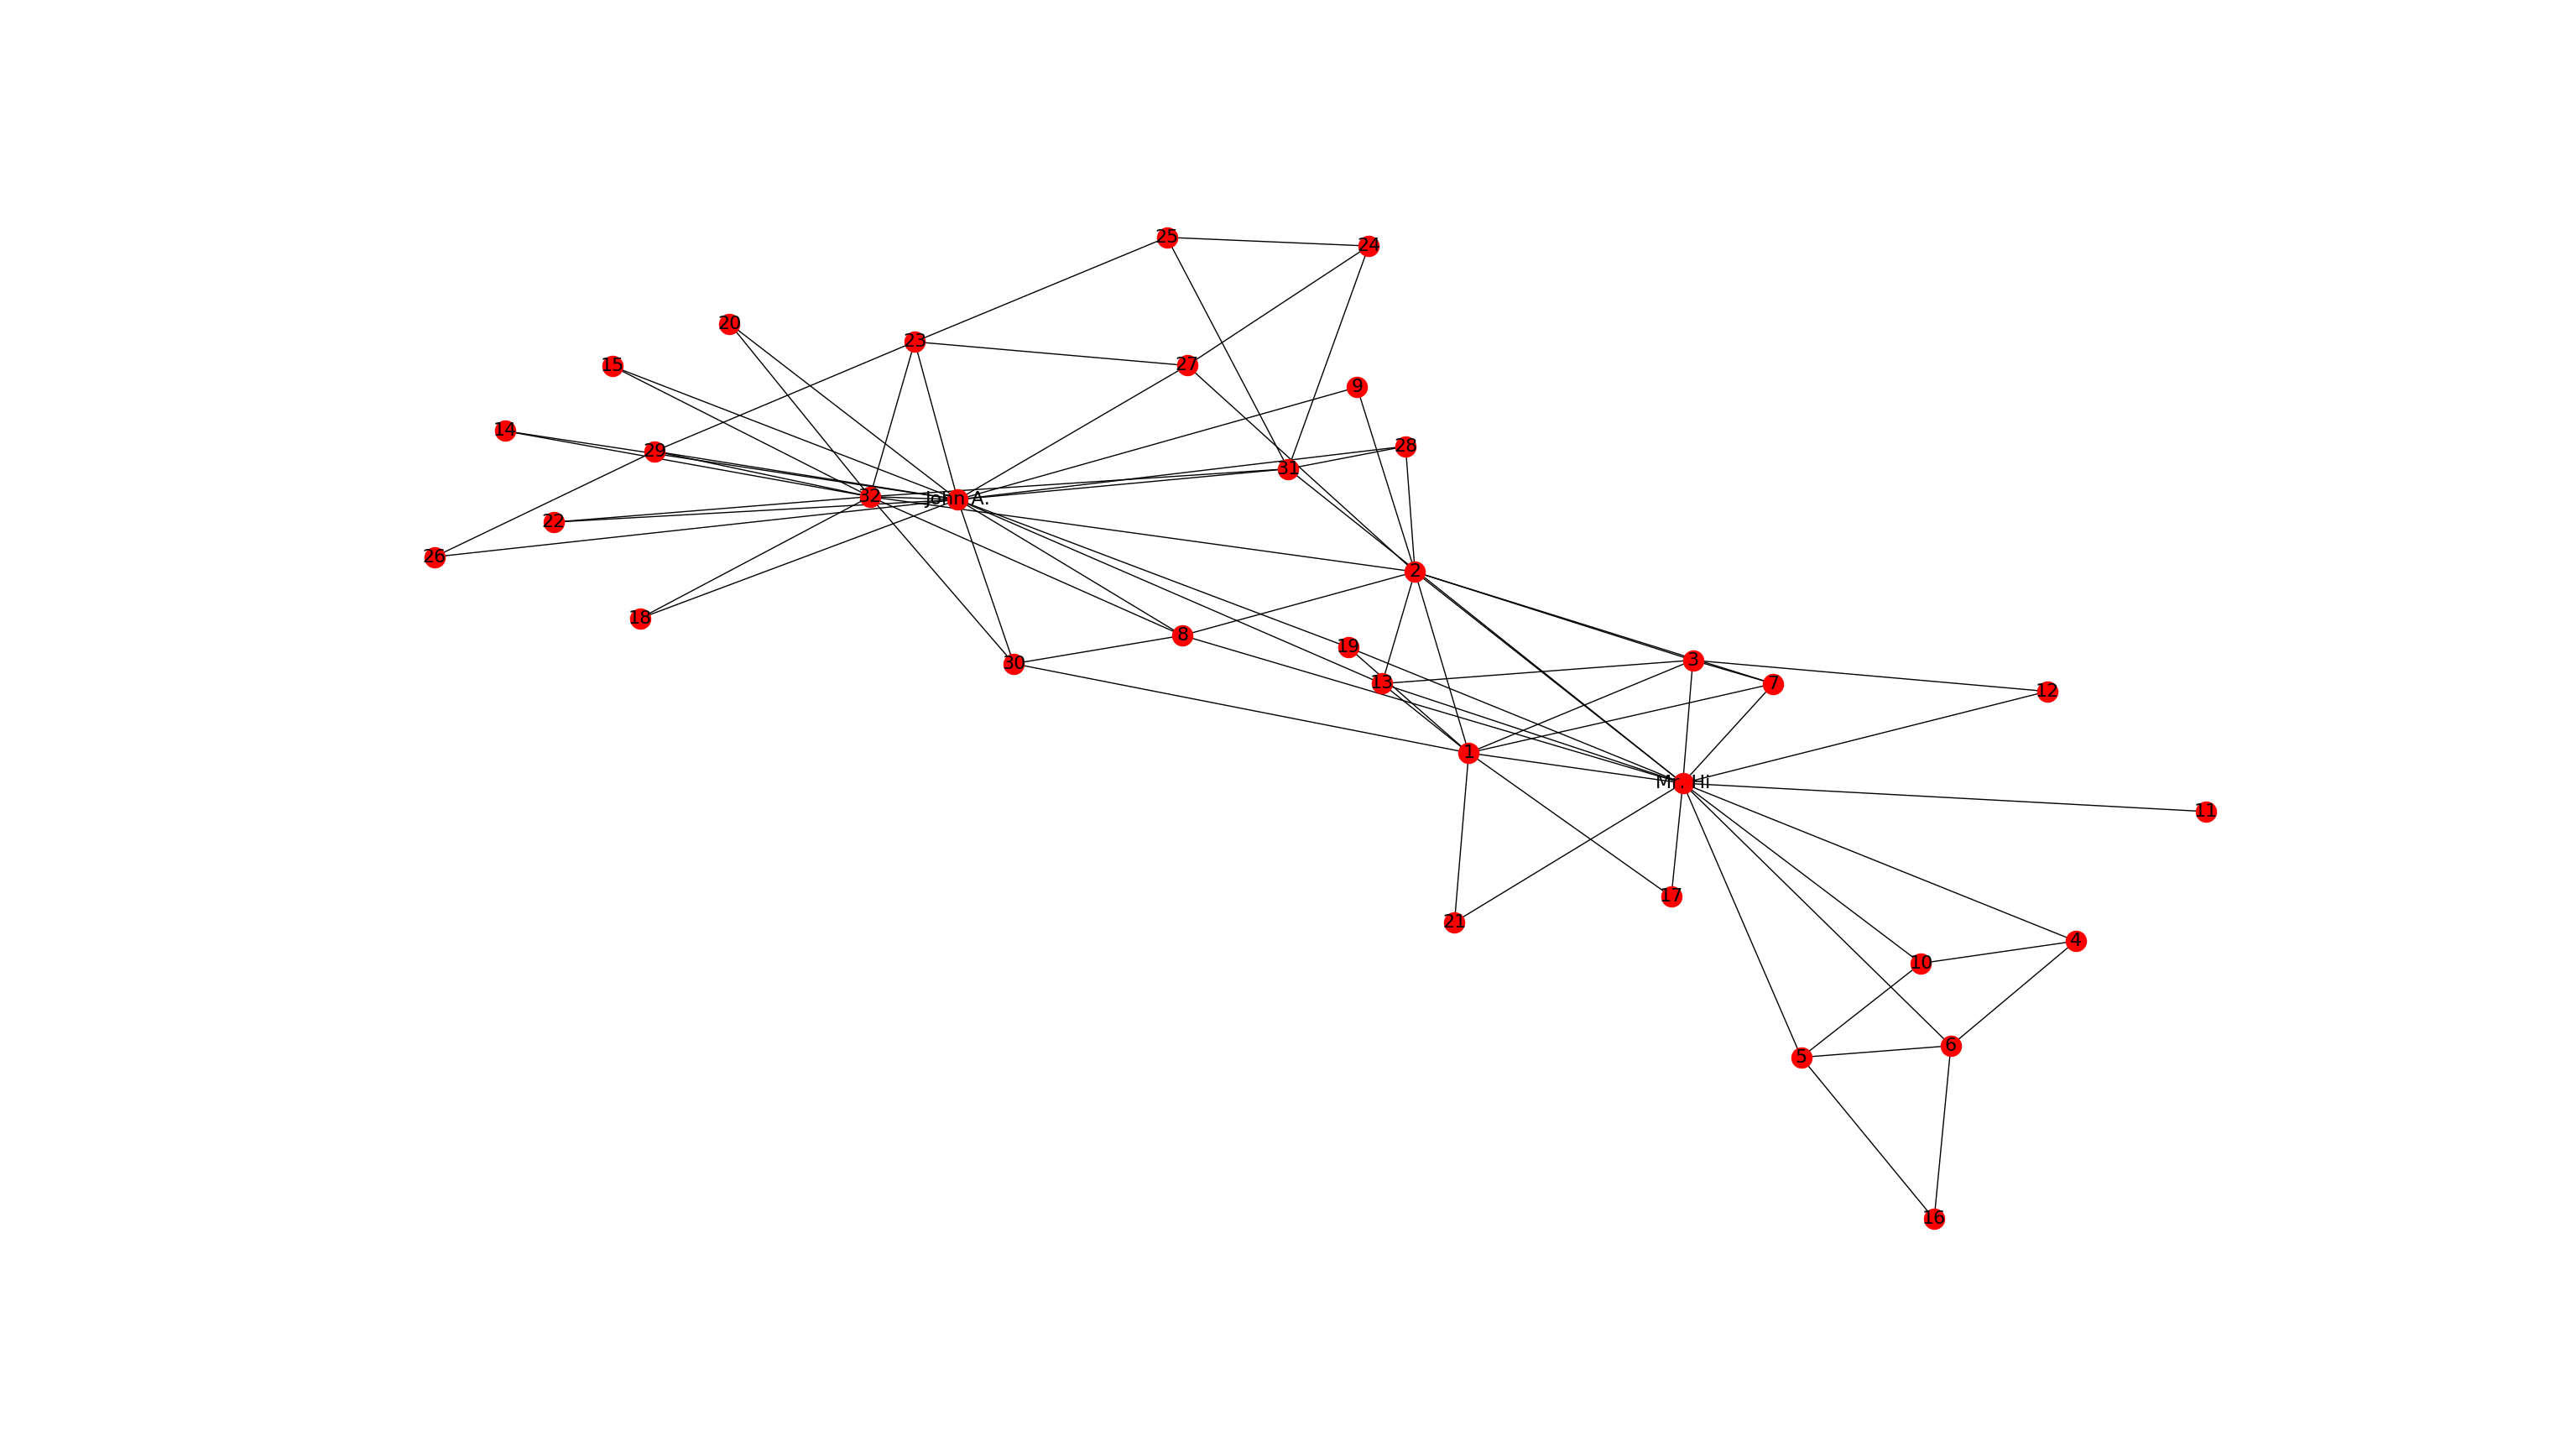
\includegraphics[width=0.9\textwidth]{Connected.png}
  \caption{Connected Karate Club}
  \label{KarateClub}
\end{figure}

\begin{lstlisting}[language=python, breaklines=true]
def most_central_edge(G):
    centrality = nx.edge_betweenness_centrality(G, weight='weight')
    return max(centrality, key=centrality.get)


def disconnected_graph():
    G = nx.karate_club_graph()
    print("Node Degree")
    for v in G:
        print('%s %s' % (v, G.degree(v)))
    comp = girvan_newman(G,most_valuable_edge=most_central_edge)
    partition_dict = {}
    list_items = []
    for c in next(comp):
        print(c)
        list_items.append(list(c))
    for items in list_items:
        for i in items:
            partition_dict[i] = list_items.index(items)

    print(partition_dict)


    labels = {}

    for i in range(0, G.number_of_nodes()):
        labels[i] = i
        if i == 0:
            labels[i] = "Mr. Hi"
        elif i == 33:
            labels[i] = "John A."

    pos = nx.spring_layout(G)
    nx.draw_networkx_nodes(G, pos, node_size=600 ,cmap=plt.cm.RdYlBu, node_color=list(partition_dict.values()))
    nx.draw_networkx_edges(G, pos, alpha=0.3)
    nx.draw_networkx_labels(G, pos, labels,font_size=16)

    plt.axis('off')
    plt.show()
\end{lstlisting}


\begin{figure}[ht]
  \centering
  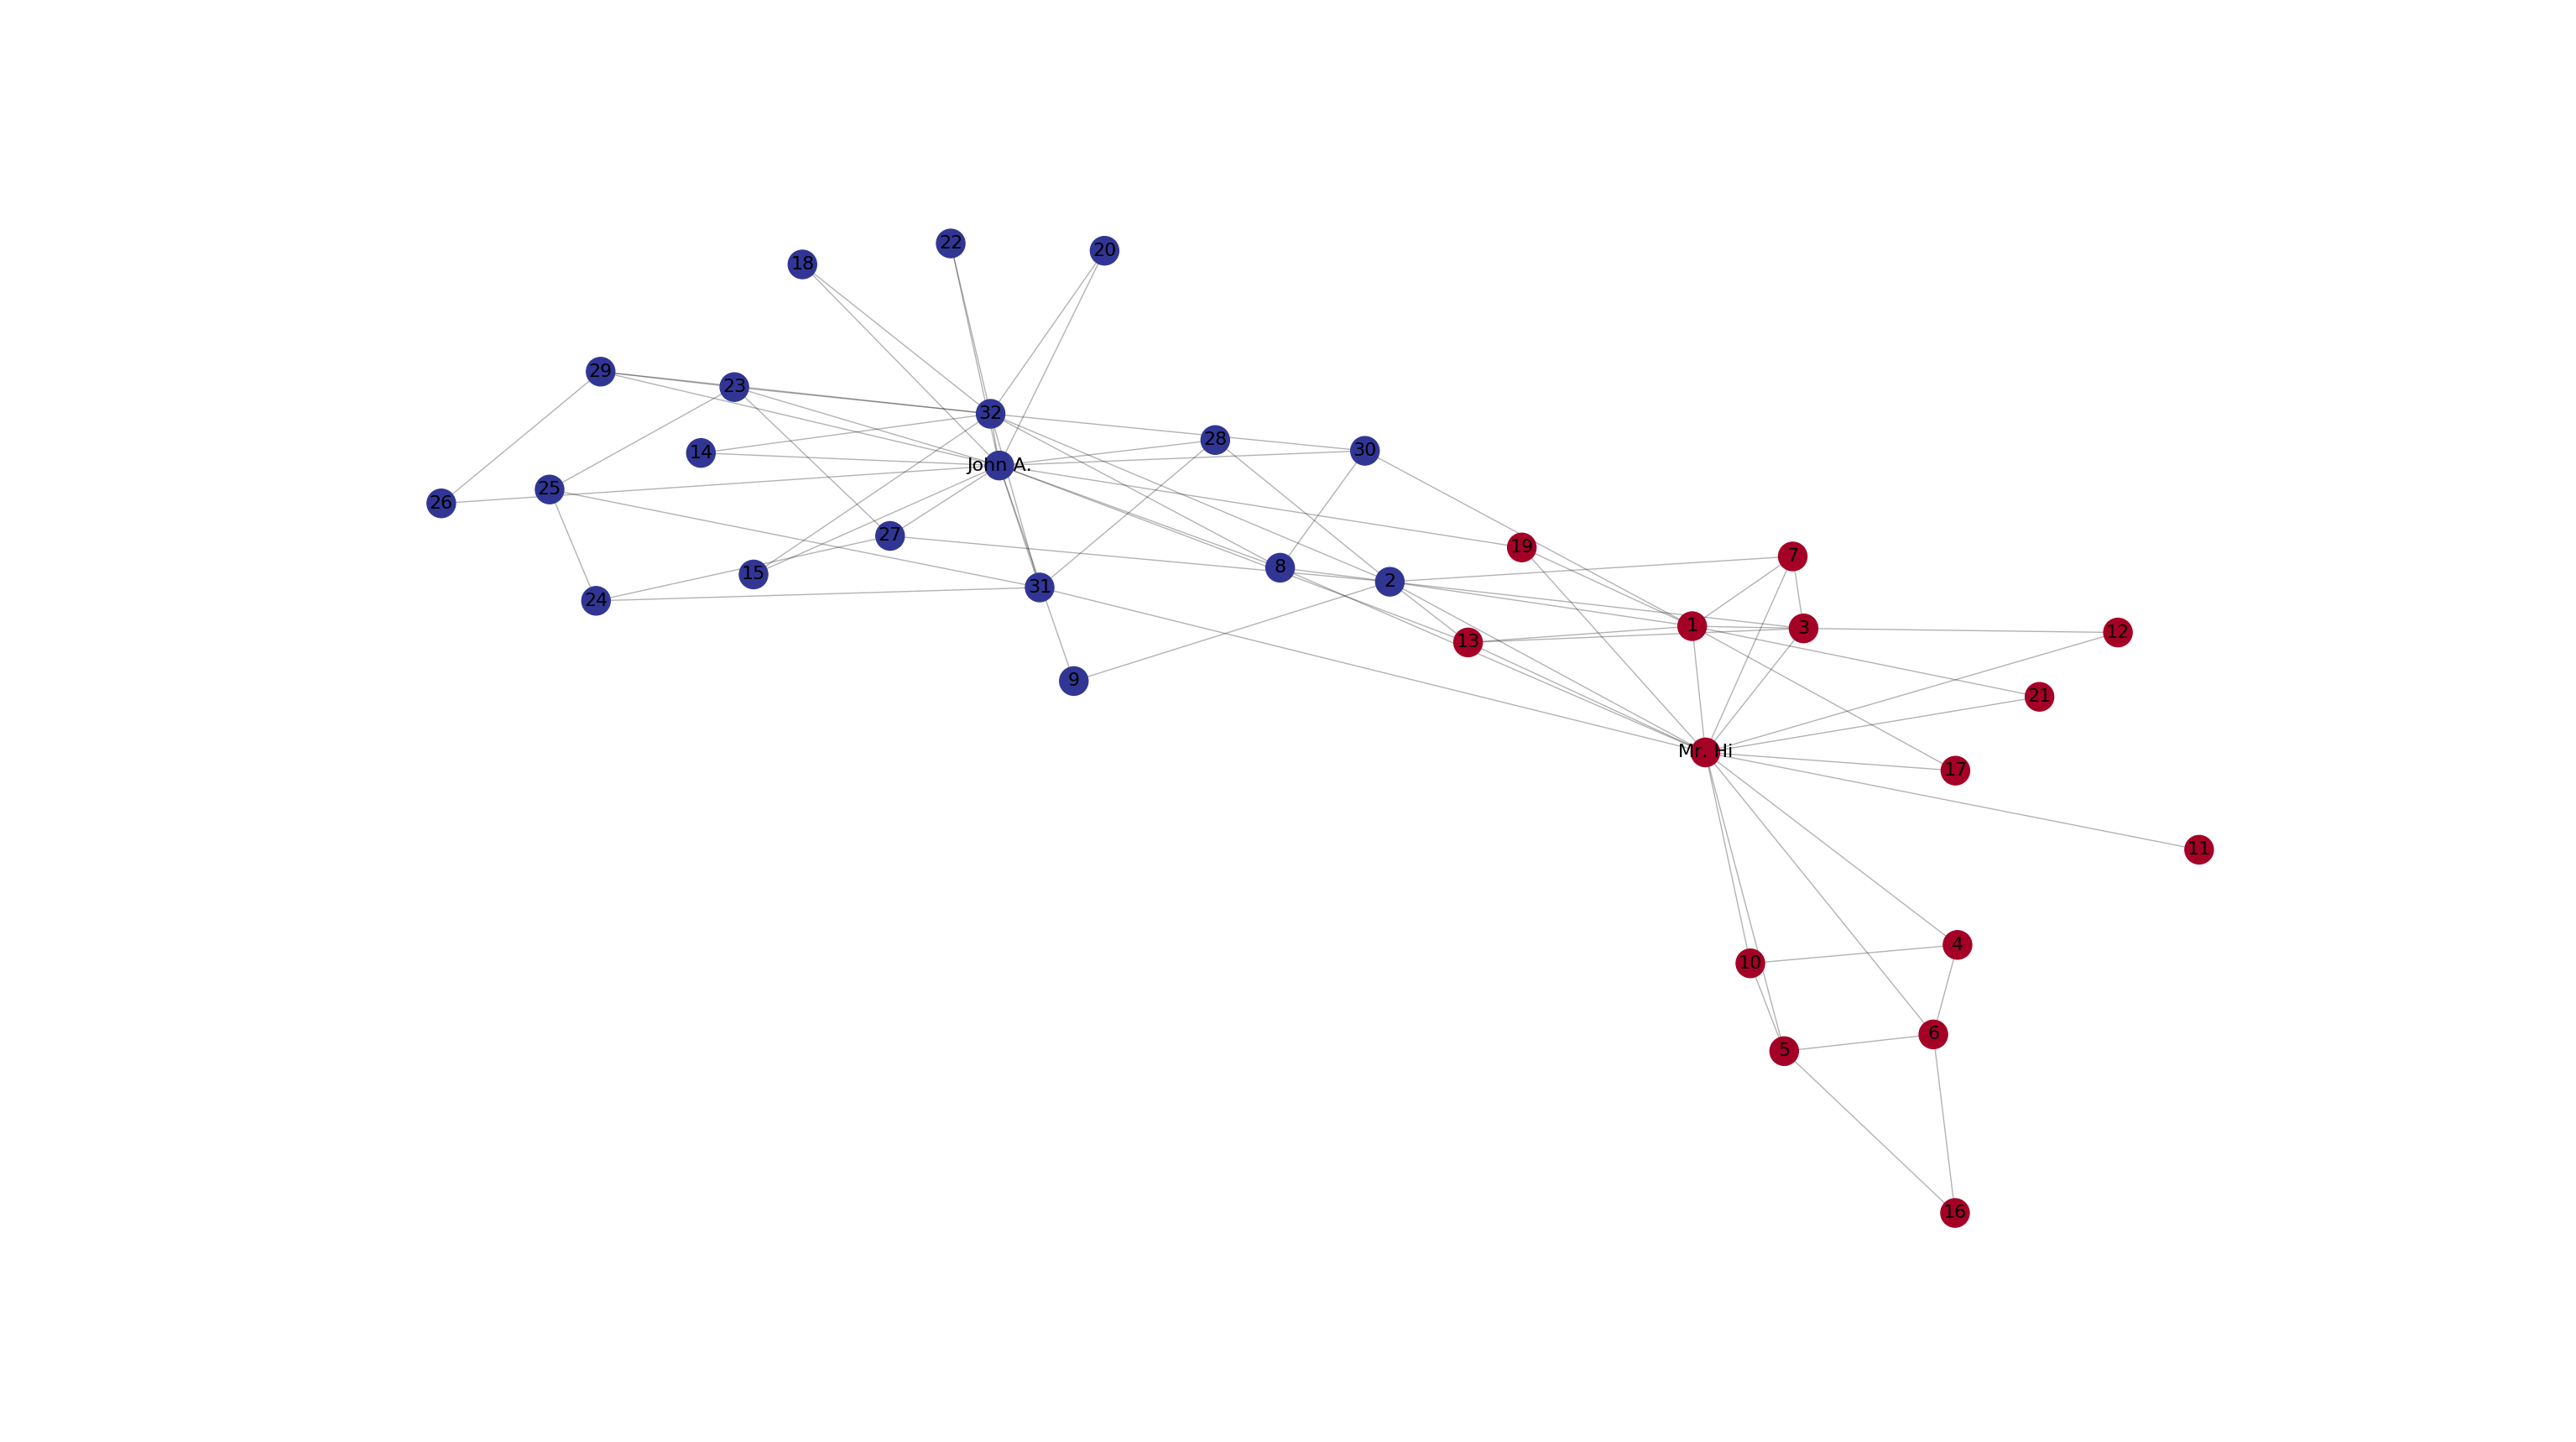
\includegraphics[width=0.9\textwidth]{Girvan.png}
  \caption{Karate Club graph showing affinity of nodes to each source, where blue nodes support John A. and red nodes support Mr. Hi}
  \label{SplitClub}
\end{figure}

\begin{lstlisting}[language=python, breaklines=true]
def multiple_iterations():
    G = nx.karate_club_graph()
    print("Node Degree")
    for v in G:
        print('%s %s' % (v, G.degree(v)))
    # comp = girvan_newman(G,most_valuable_edge=most_central_edge)
    comp = girvan_newman(G)
    comp1 = girvan_newman(G)
    comp2 = girvan_newman(G)
    list_items = []
    for c in comp:
        list_temp = []
        for itr in c:
            list_temp.append(list(itr))
        list_items.append(list(list_temp))
    counter = 0
    for items in list_items:
        print("Iteration")
        partition_dict = {}
        for i in items:
            for j in i:
                partition_dict[j] = items.index(i)
        print(partition_dict)
        temp_G = copy.deepcopy(G)
        print(temp_G.edges())
        for key_i in partition_dict:
            for key_j in partition_dict:
                if temp_G.has_edge(key_i, key_j) and partition_dict[key_i] != partition_dict[key_j]:
                    temp_G.remove_edge(key_i, key_j)
        labels = {}
        print(temp_G.edges())
        for i in range(0, temp_G.number_of_nodes()):
            labels[i] = i
            if i == 0:
                labels[i] = "Mr. Hi"
            elif i == 33:
                labels[i] = "John A."
        if counter > 1:
            figure(figsize=(20, 20))
        else:
            figure(figsize=(15, 15))
        pos = nx.spring_layout(temp_G)
        nx.draw_networkx_nodes(temp_G, pos, node_size=600, cmap=plt.cm.RdYlBu, node_color=list(partition_dict.values()))
        nx.draw_networkx_edges(temp_G, pos, alpha=0.3)
        nx.draw_networkx_labels(temp_G, pos, labels, font_size=16)

        plt.axis('off')
        file_name = "Girvan_Newman" + str(counter) + ".png"
        plt.savefig(file_name)
        if counter < 4:
            counter = counter + 1
        else:
            exit()
\end{lstlisting}


\begin{figure}[ht]
  \centering
  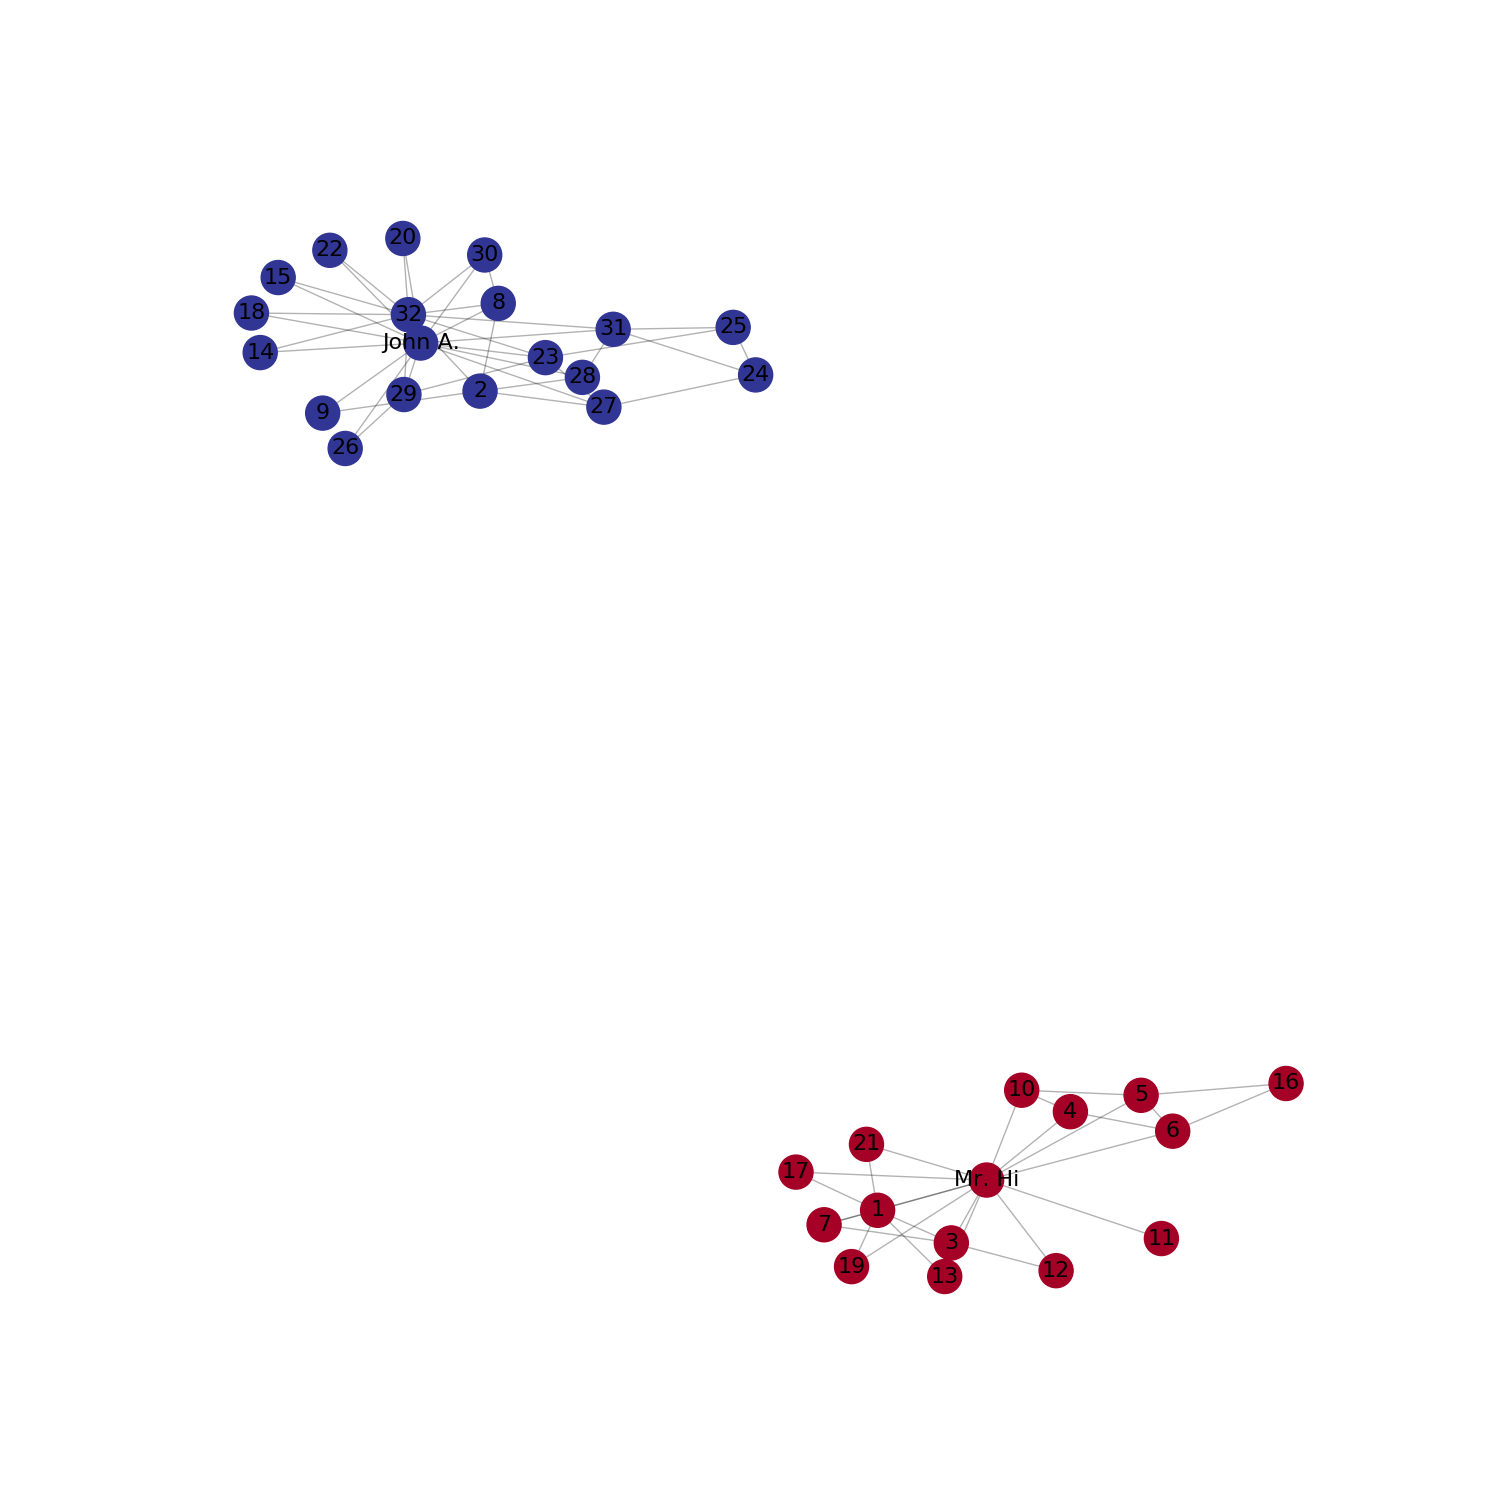
\includegraphics[width=0.9\textwidth]{GirvanNewman0.png}
  \caption{Two connected components from the Karate Club graph}
  \label{Girvan}
\end{figure}
\end{enumerate}
  
%}

\end{homeworkProblem}

%----------------------------------------------------------------------------------------
%   PROBLEM 2
%----------------------------------------------------------------------------------------

\begin{homeworkProblem}

We know the group split in two different groups.  Suppose the disagreements in the group were more nuanced -- what would the clubs look like if they split into groups of 3, 4, and 5?
%\problemAnswer
%{
    \begin{verbatim}\end{verbatim}
    \textbf{SOLUTION}\\
 If the group splits become more nuanced, the group split for 3 would look like the network graph in figure \ref{Split3}. Similarly for split into 4 incan be viewed in figure \ref{Split4}, split for 5 in figure \ref{Split5} ,and split for 6 in figure \ref{Split6}. 

\begin{figure}[ht]
  \centering
  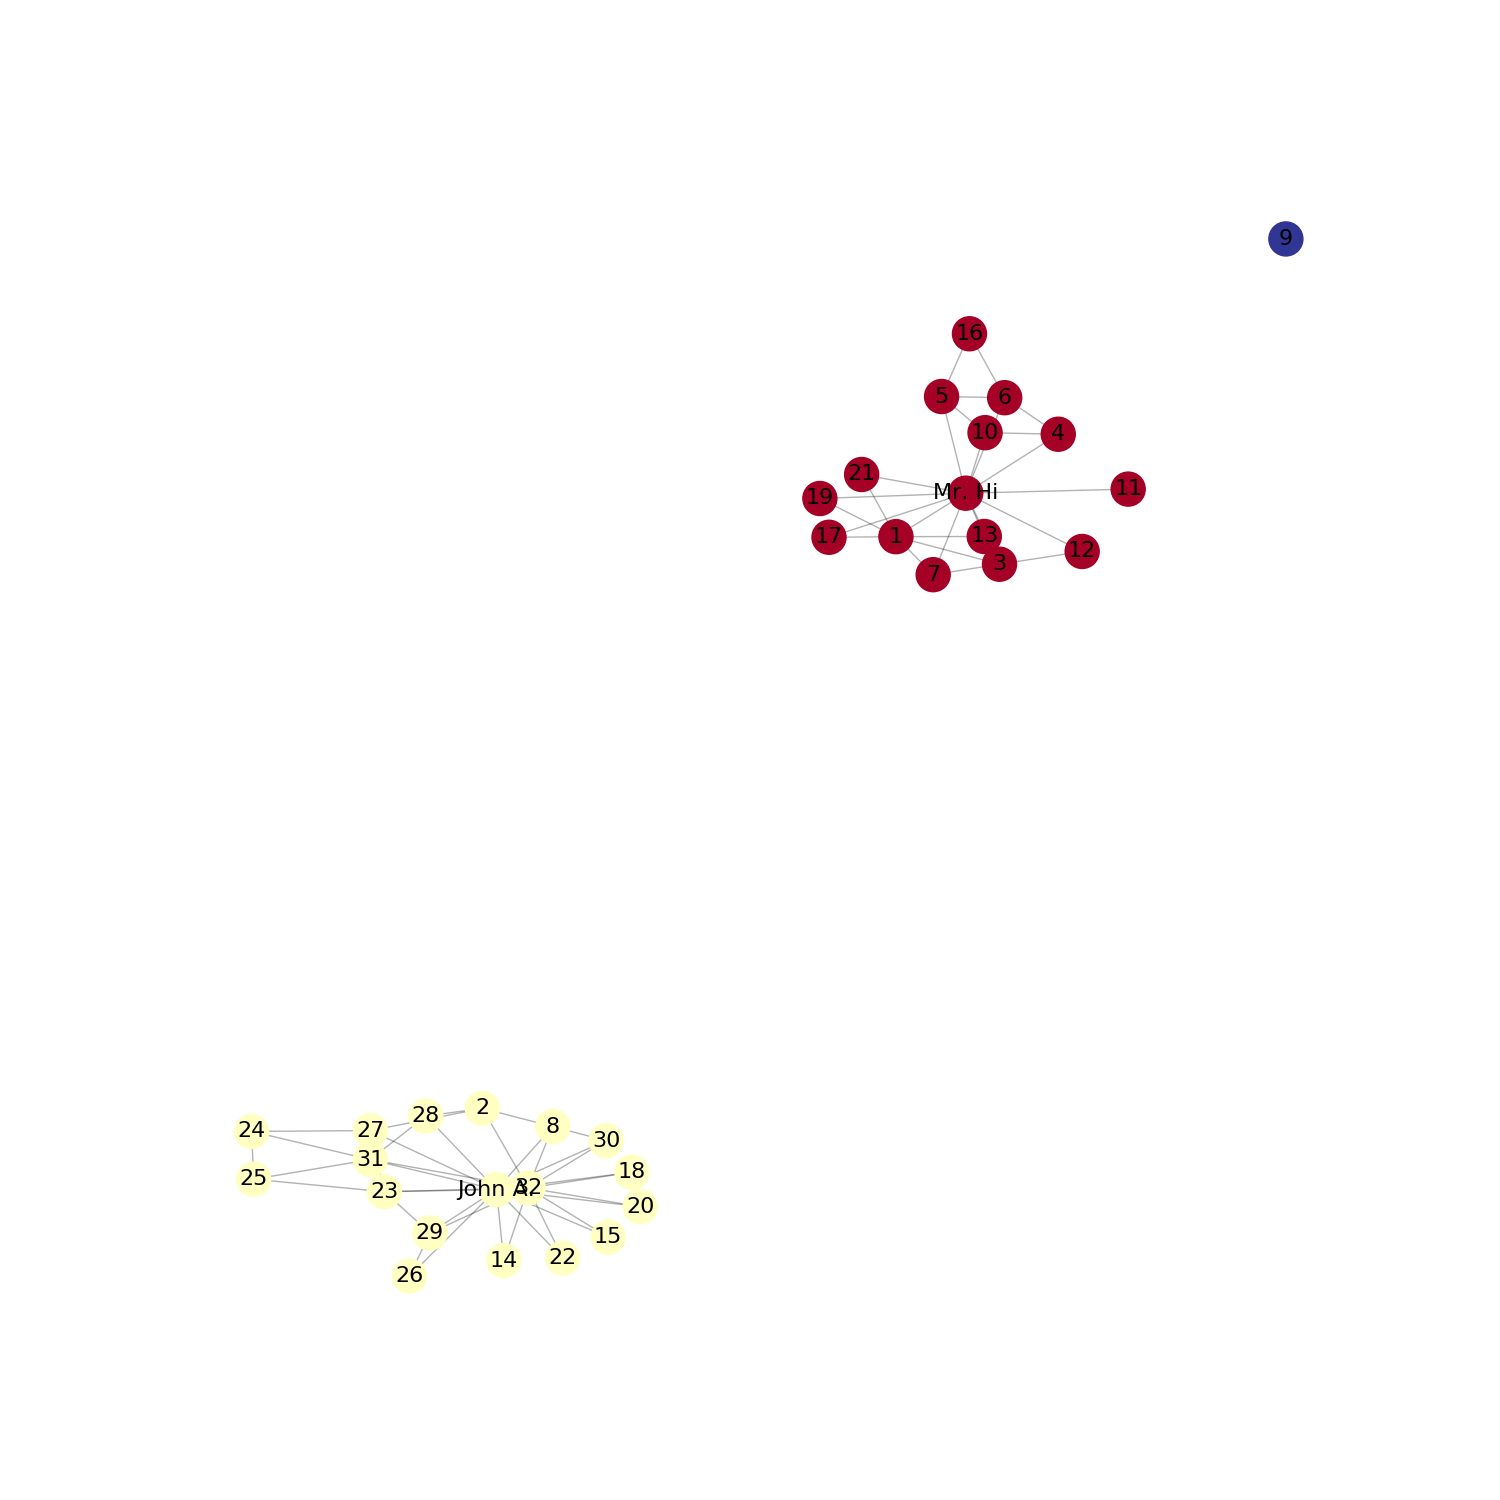
\includegraphics[width=0.9\textwidth]{GirvanNewman1.png}
  \caption{Karate Club split in 3 groups}
  \label{Split3}
\end{figure}

\begin{figure}[ht]
  \centering
  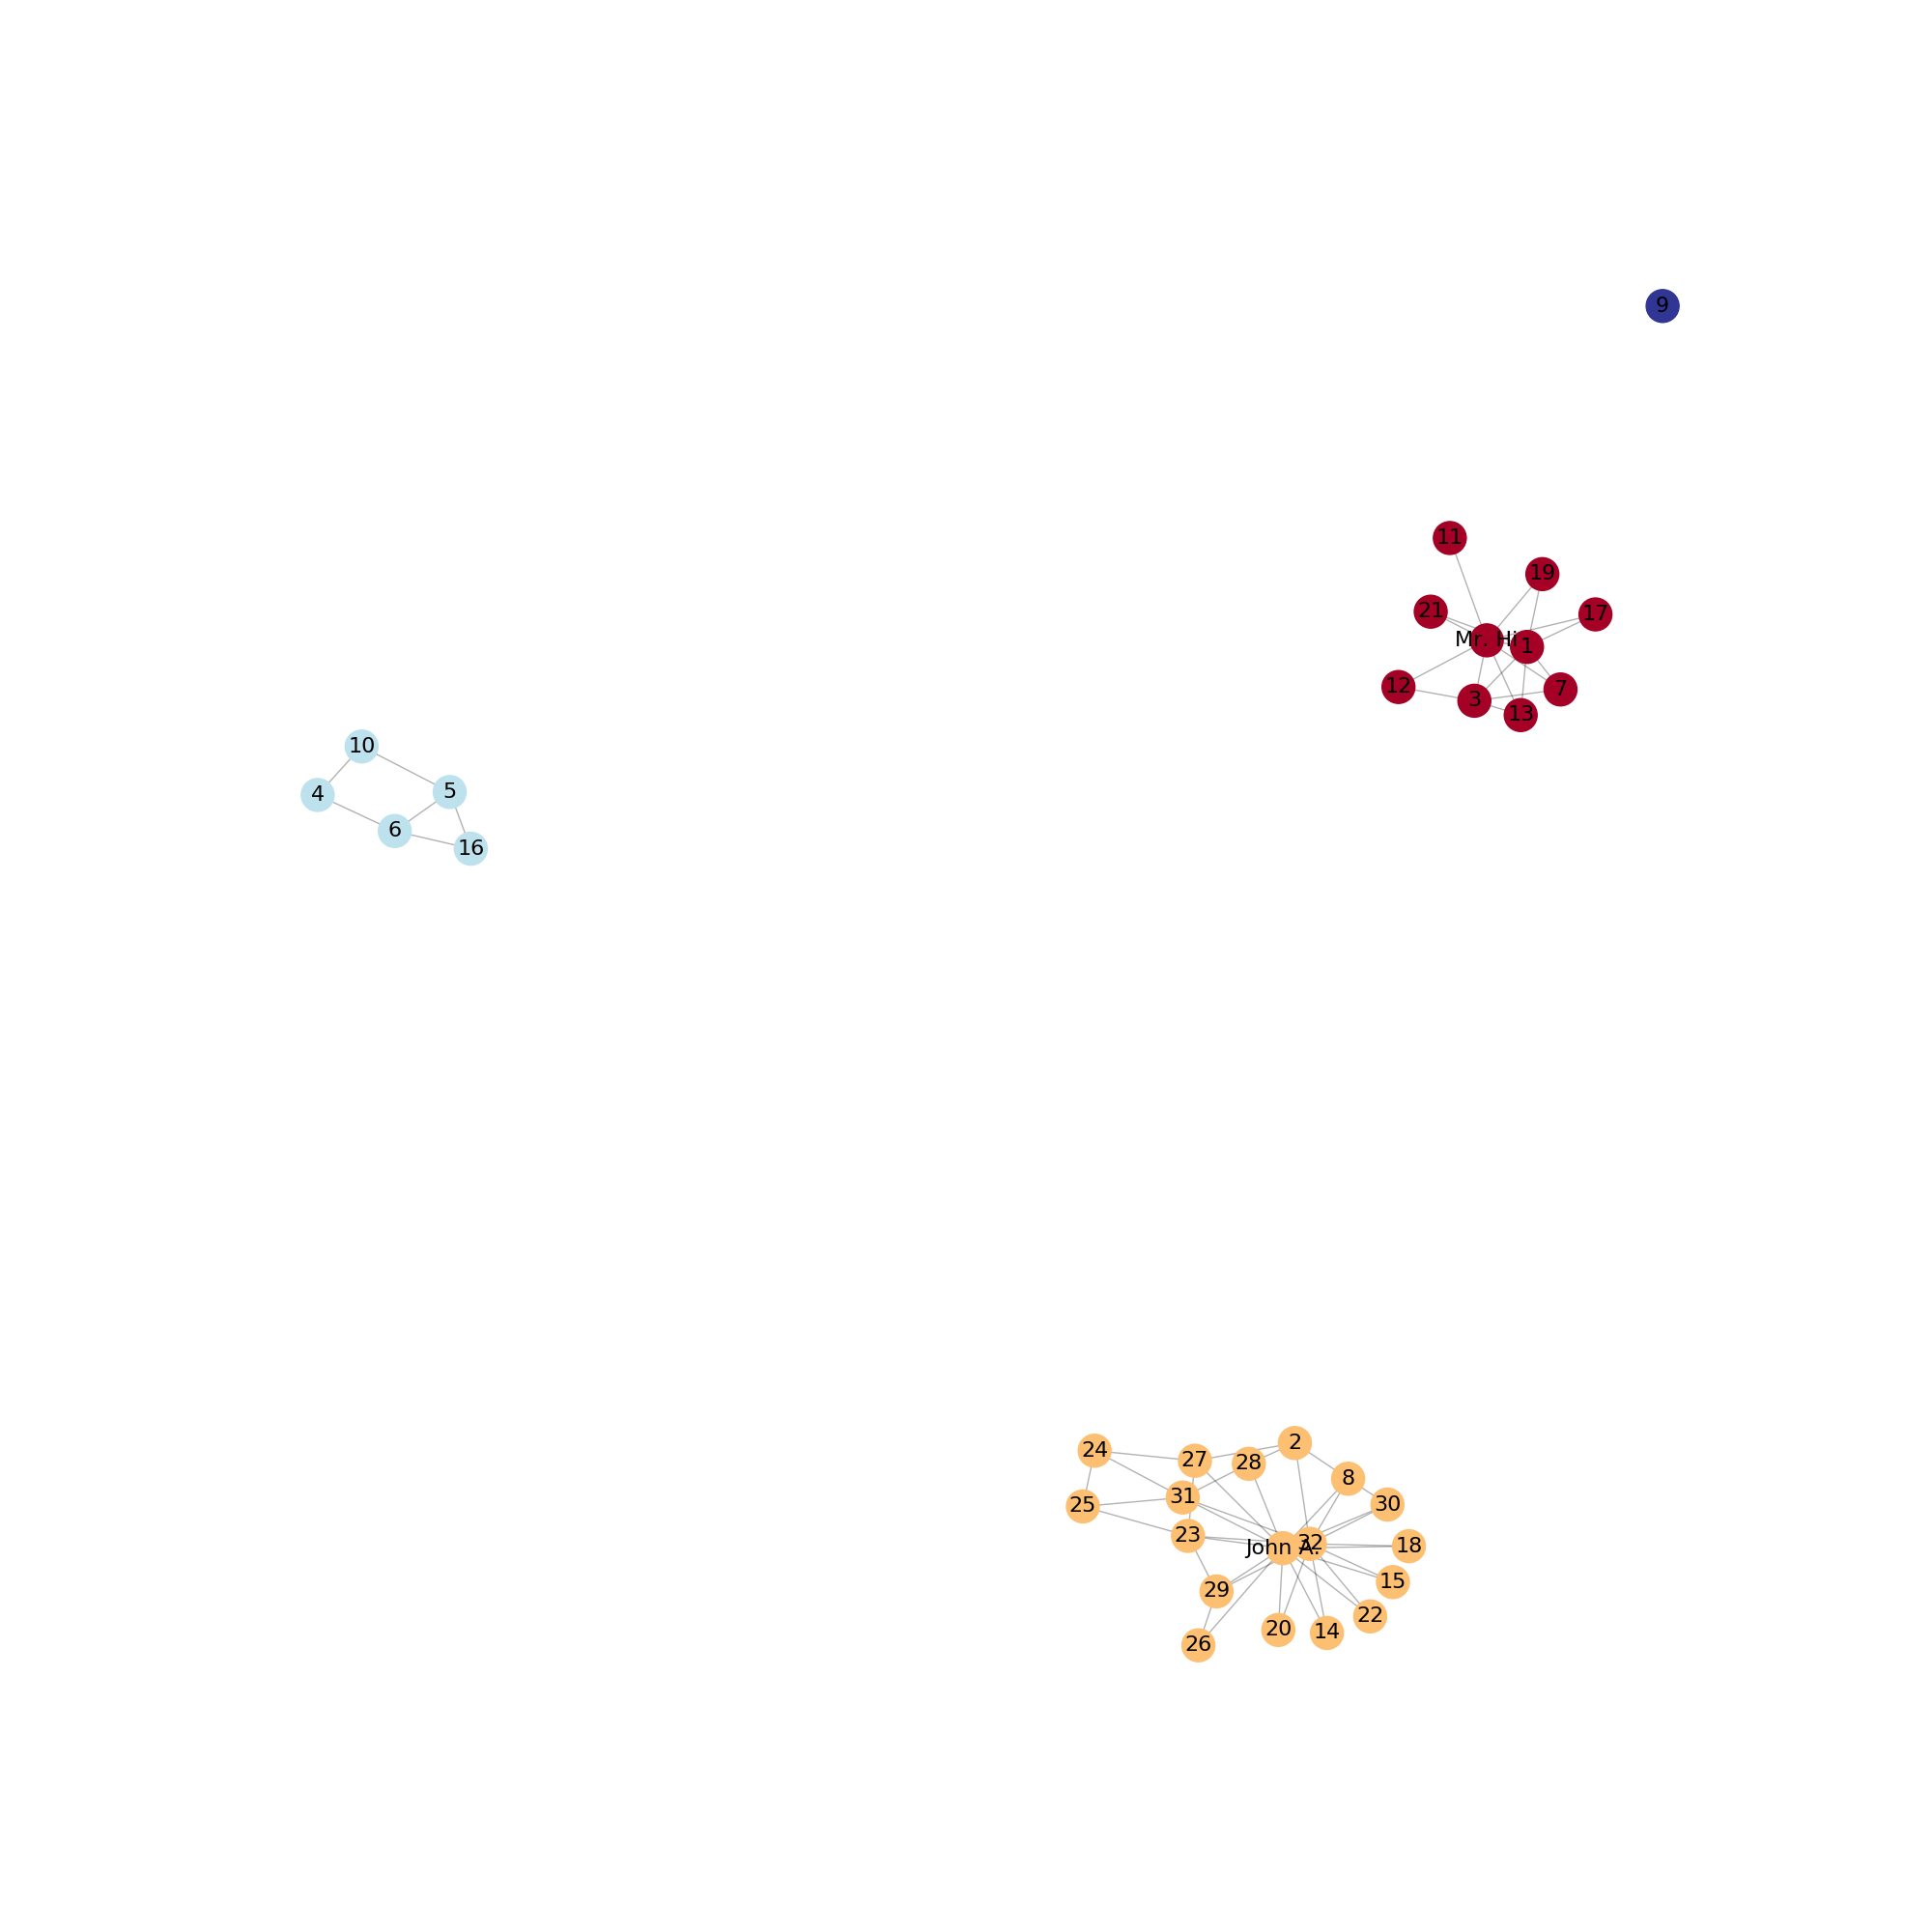
\includegraphics[width=0.9\textwidth]{GirvanNewman2.png}
  \caption{Karate Club split in 4 groups}
  \label{Split4}
\end{figure}
\begin{figure}[ht]
  \centering
  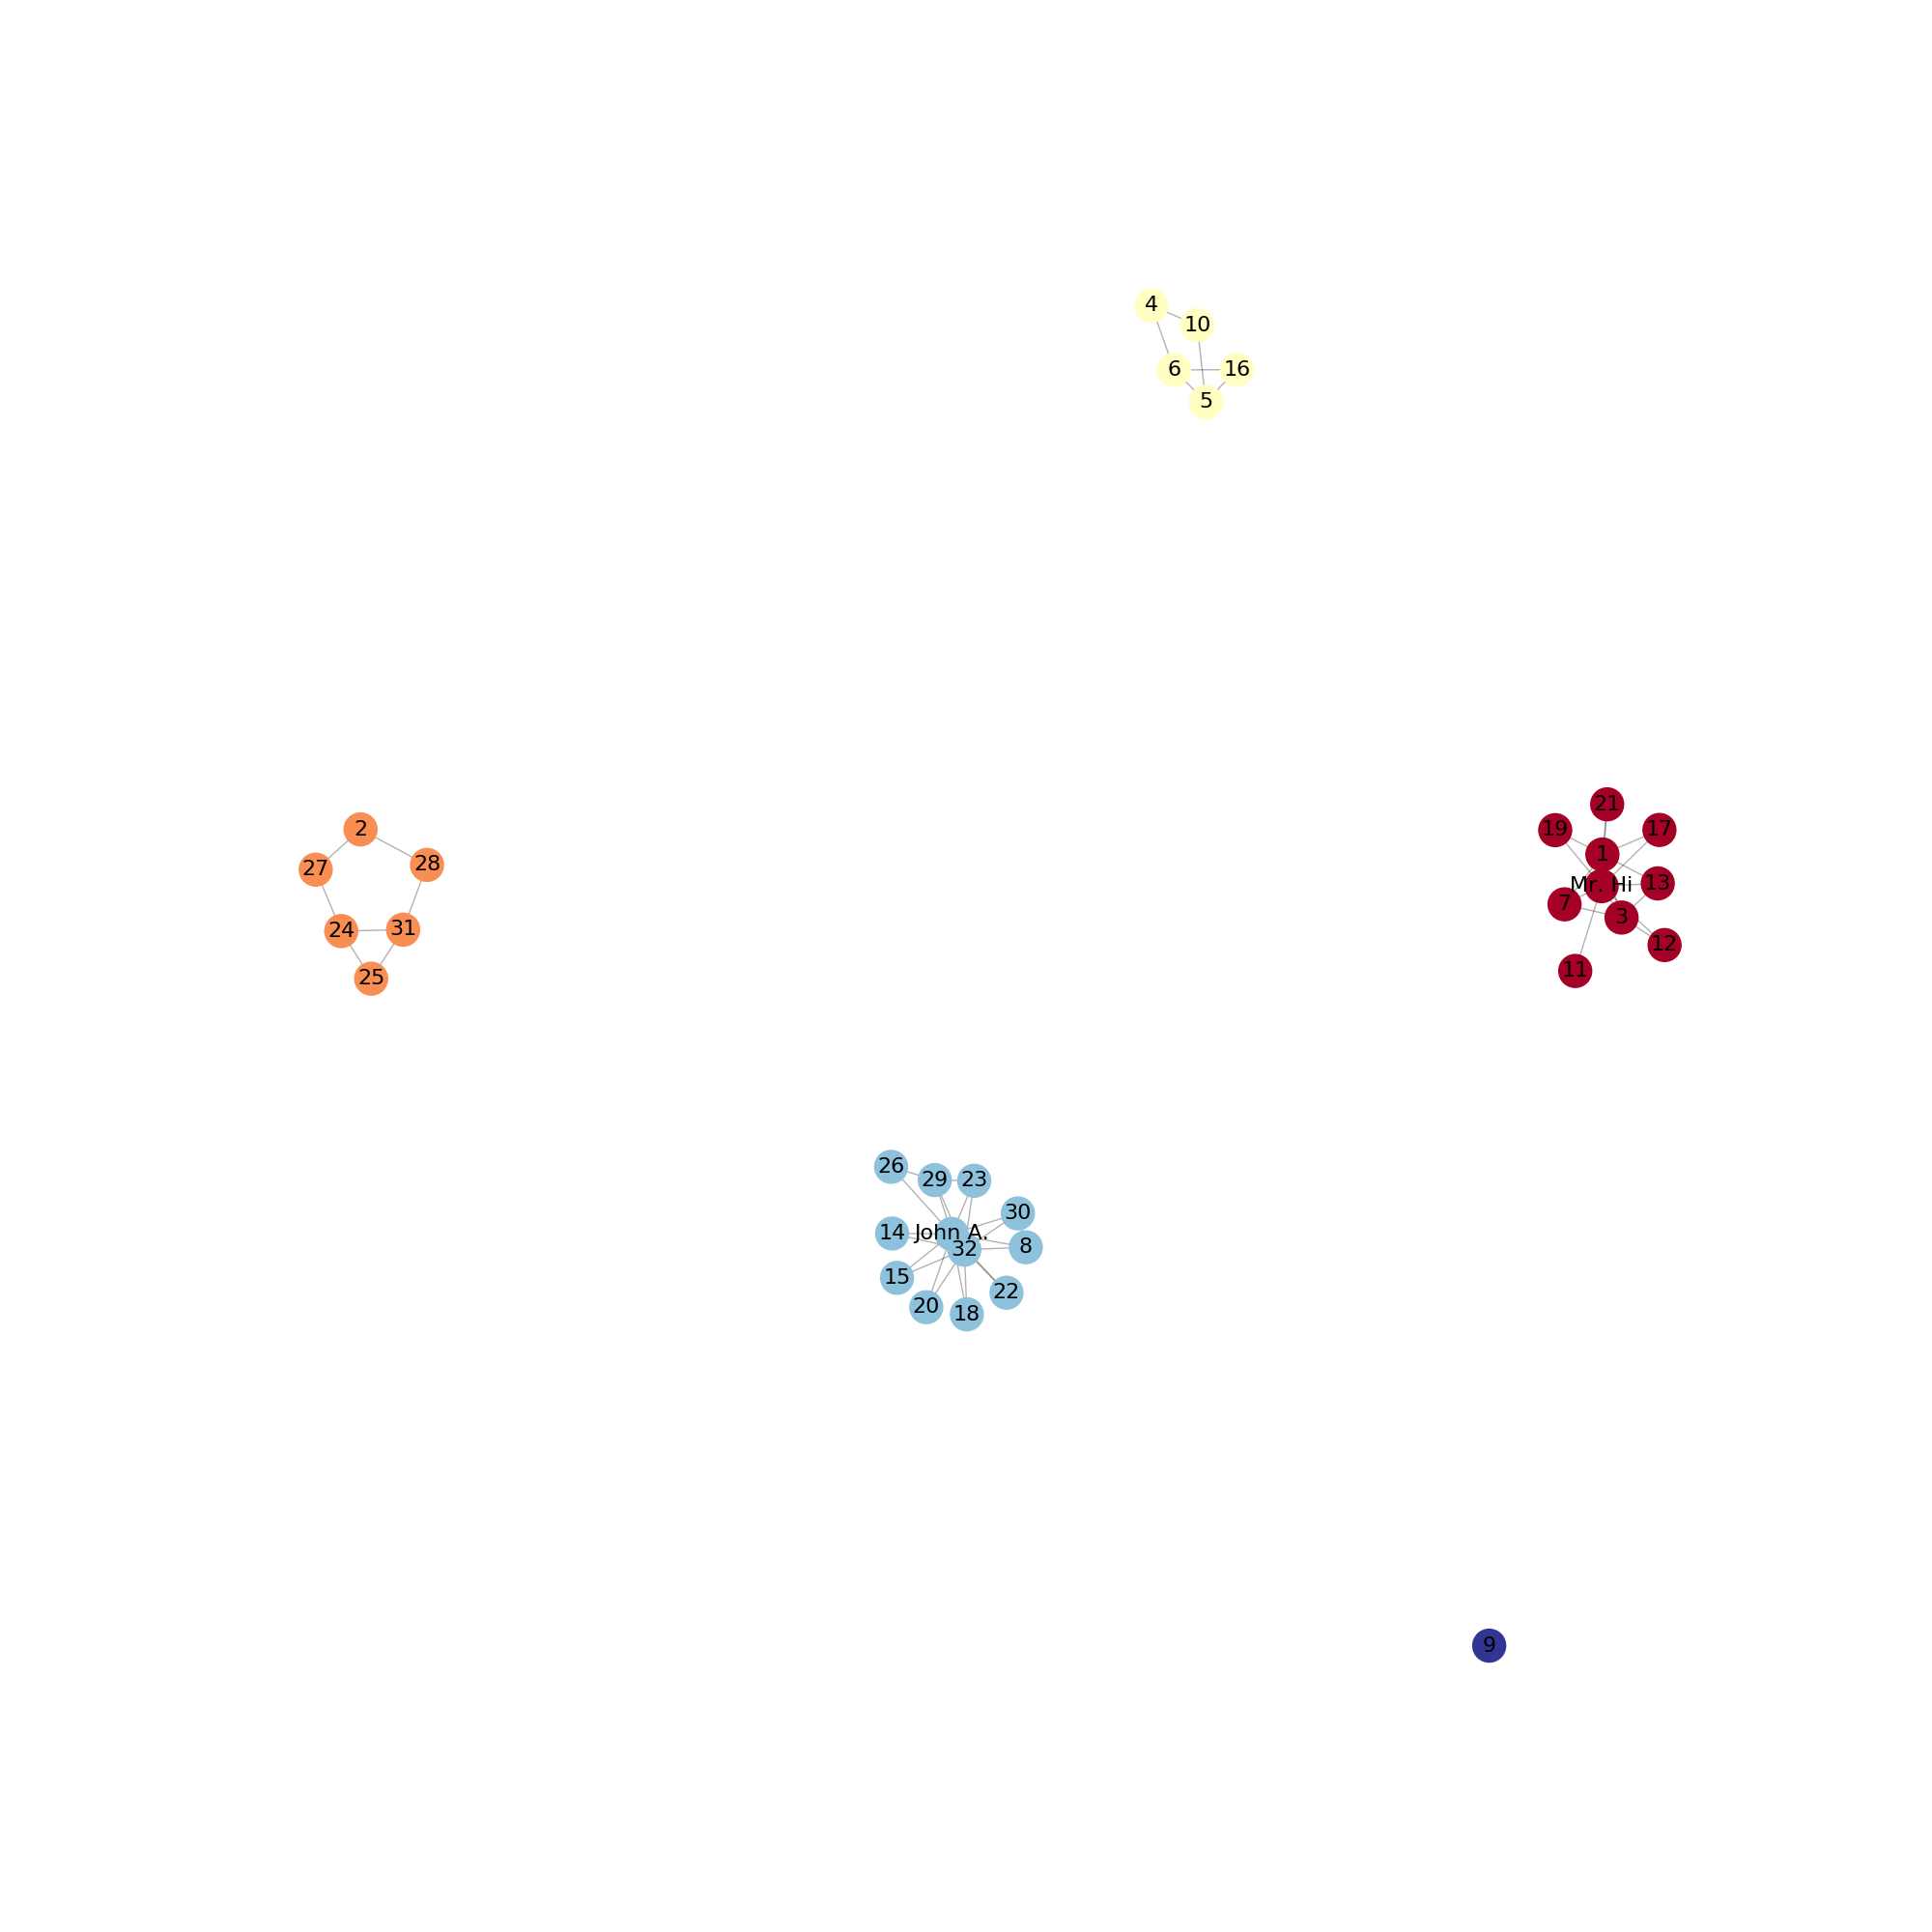
\includegraphics[width=0.9\textwidth]{GirvanNewman3.png}
  \caption{Karate Club split in 5 groups}
  \label{Split5}
\end{figure}
\begin{figure}[ht]
  \centering
  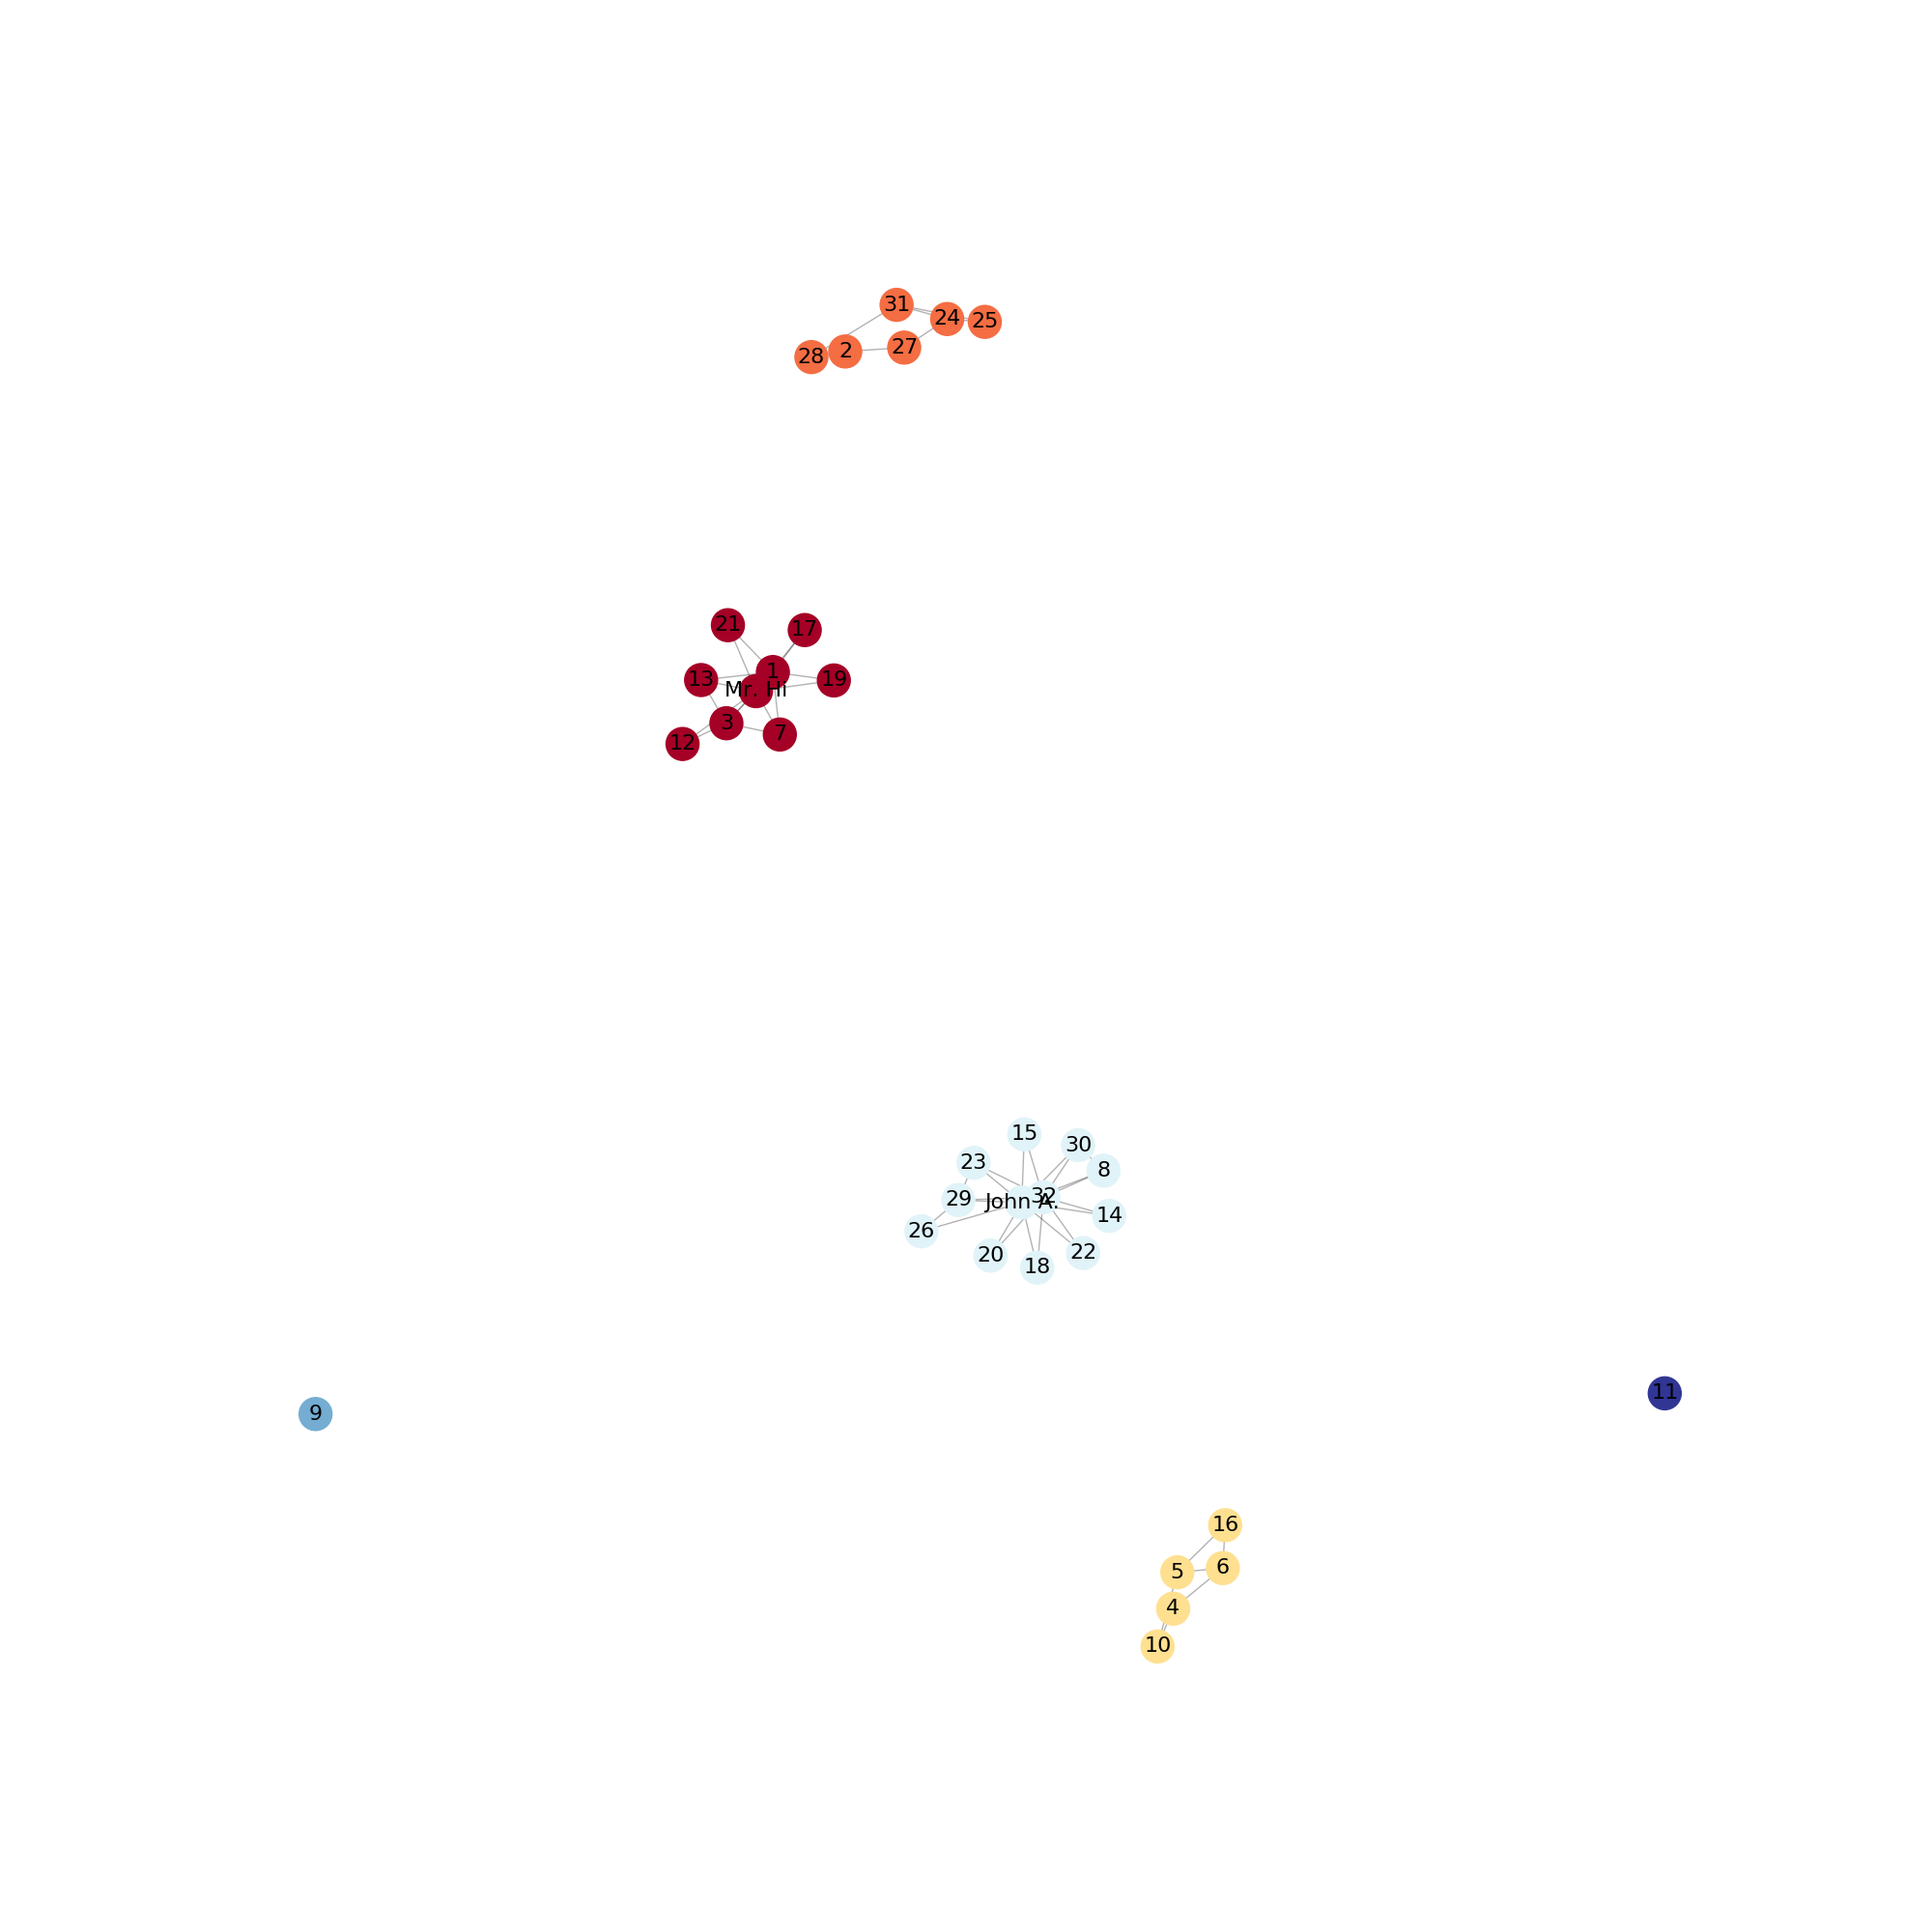
\includegraphics[width=0.9\textwidth]{GirvanNewman4.png}
  \caption{Karate Club split in 6 groups}
  \label{Split6}
\end{figure}

%}

\end{homeworkProblem}


\end{document}
    


   

    

    

    
   
